\section{The Design Space of Pipes}
The design space of pipes has four dimensions: openings, design focus, topologies, and inserted media.  We describe the space below.

\begin{figure}[h!]
\centering
    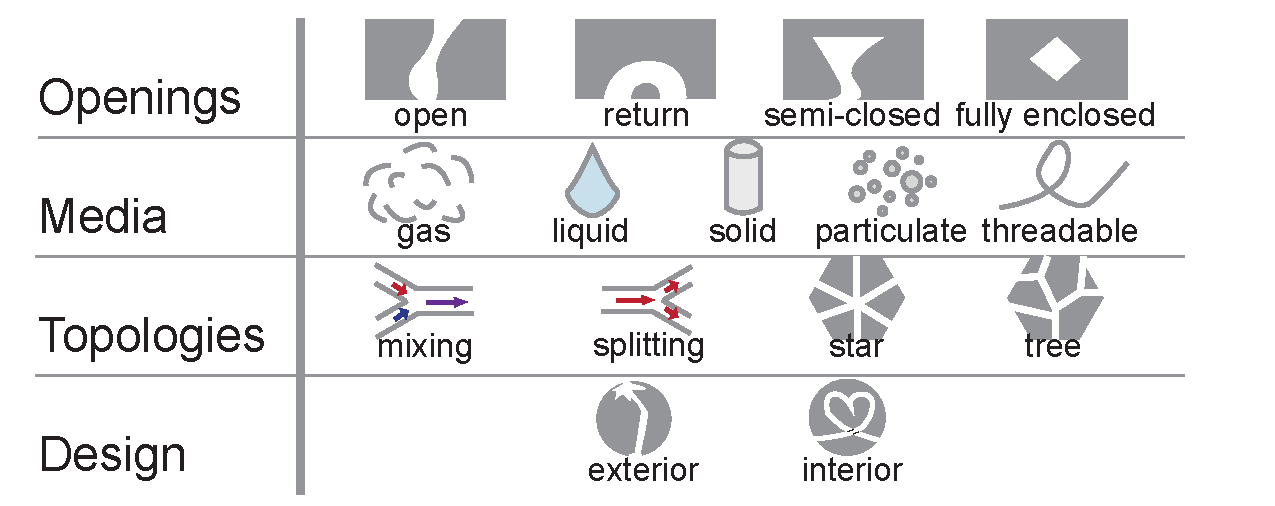
\includegraphics[width=3.4in]{figures/tubespace.pdf}
\caption{The design space of pipes.  See text for details.}
\label{fig:pipespace}
\end{figure}

\subsection{Openings of Pipes}

\george{difference between open/return not clear}Pipes can have four opening styles: open, return, semi-closed, and fully enclosed (see Figure \ref{fig:pipespace}).  As we are interested in interactive devices, we distinguish a ``user side"---part of the surface or interior of an object facing its user for interaction; and a ``system side"---where other hardware such as electronics may be connected.  We refer to a pipe which is ``open on the user side'' to have its contents \emph{physically accessible} to a user \emph{at interaction time}.  ``Closed on the user side'' implies physically cut off from the user.  Similarly with the system side.  User or system manipulation of pipe contents are possible even without physical access, e.g., via soundwaves. \george{confusing}

\begin{figure}[h]
\centering
    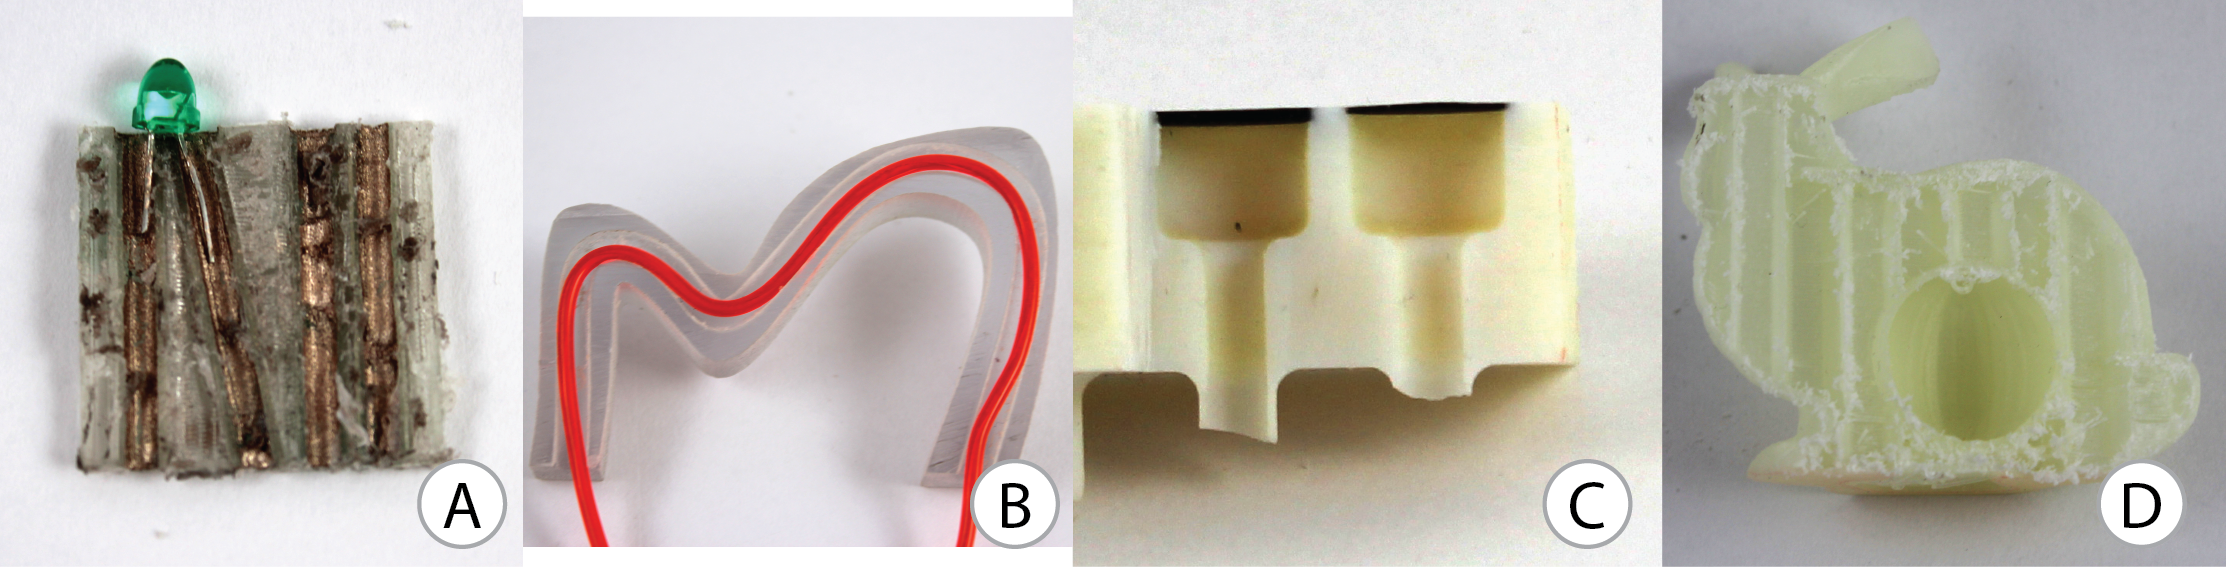
\includegraphics[width=3.4in]{figures/types.png}
\caption{Pipe openings: A shows a pair of open tubes filled with copper paint to power an LED.  B shows a return pipe with EL wire threaded through it.  C shows two semi-closed pipes capped by rubber membranes.  In D, a rabbit has a fully enclosed chamber to modify its weight.}
\label{fig:openings}
\end{figure}

Open pipes originate from the system side and connect the user side, with both ends of the pipe open. This type of pipe may be used to create electronic circuitry.  For example, an open pipe filled with conductive paint can power an LED (see Figure \ref{fig:openings}A).

A return pipe originates at the system and returns back to it, without offering physical access to the user.  By threading an electroluminescent (EL) wire through a clear return pipe, a maker can create a custom piece of neon art (see Figure \ref{fig:openings}B). \george{not sure this is adding something useful}

Semi-closed pipes are open on the system side, closed on the user side. A potential use of this is to create tactile output: The closed interface may be fabricated from a malleable material, e.g., a rubber membrane, and the open end attached to a fluid pump to create haptic feedback (see Figure \ref{fig:openings}C).

A fully enclosed pipe is closed to both the system and the user.  Fully enclosed pipes may be used as weight modifiers (e.g., for object identification), as in Figure \ref{fig:openings}D.  They can also contain for water or particles that would otherwise fall out.

\subsection{Design of Pipes}
Pipe design may emphasize exterior connection points and/or interior paths.  Our maze (see Figure \ref{fig:maze}) requires specific terminals (the start and end of the maze) as well as a specific path for its tubes (the maze itself).  Alternatively, the neon sign's output in Figure \ref{fig:neon} is based only on the \emph{path} of the pipe.  Focused on just the exterior features is the touch sensitive toy in Figure \ref{fig:toys}, where pipes must exit the toy at the frontal lobe and parietal lobes to make those \emph{specific locations} touch-sensitive.  A pipe for weight modification does require specific terminals or a specific path (see Figure \ref{fig:openings}D).

\subsection{Pipe Topologies}

Pipe network topologies enable different interactions \george{how?}.  Splitting or mixing pipes offer flexibility in output, allowing a single source to have multiple outputs or multiple sources to combine (see Figure \ref{fig:pipespace}).  Star and tree topologies extend the splitting and mixing primitives, encompassing multiple-in and multiple-out in contrast to single-in/single-out; we used star topologies in our toys \ref{fig:toys}.

\subsection{Media in Pipes}
After printing, there is still flexibility in inserting media to create different interface affordances and capabilities. We consider gas, liquids, solids, particulates, and threadables.

``Gas'' comprises compressible fluids.  Fluid pressure inside semi-closed pipes can create haptic feedback, or gases can be used as carriers for scents or fog; fluid pressure can also be used as an input.

Incompressible fluids (``liquids'') perform similarly to gases for display or haptics.  Additionally, using driable conductive liquids like copper paint, pipes can become custom wires.

Pipes need not have hollow centers: in the case where routed pipes are filled with solid material---in particular, a solid material different from the enclosing model material---, interactions such as those in Printed Optics \cite{Willis-printedoptics} are possible.

Particulates, either printed in-place or inserted, can be of varying densities.  A single particle can be used for display.  Sparse particles in fluid can provide haptic feedback.

Threadable media, such as EL wire or fiberoptic cables, can be threaded through pipes post-printing.  This empowers inexpensive printers: for example, a Printed Optics-style interface can be created on a consumer-grade 3D printer with pipes and fiber optic cable.
